\appendix

\section{TPF Derivation for Introspective Strided Decoding}
\label{app:tpf_derivation}

We derive the expected tokens per forward pass (TPF) for ISD at stride $N$. Let $p_k$ denote the acceptance probability of the $k$-th strided proposal, and define the cumulative acceptance probabilities $P_0 = 1$, $P_k = \prod_{j=1}^{k} p_j$ for $k \geq 1$.

Each ISD iteration consists of two forward passes: a stride step (producing $N$ candidates) and an introspection step (verifying them). The number of accepted tokens depends on where the first rejection occurs:

\begin{denseitemize}
    \item With probability $P_{N-1}$ (all proposals accepted): we obtain $N$ verified tokens plus 1 bonus token from the introspection step's logits, totaling $N + 1$ tokens from 2 forward passes.
    \item With probability $P_{k-1}(1 - p_k)$ (first rejection at position $k$, for $k = 1, \ldots, N{-}1$): we obtain $k + 1$ tokens (the quality-guaranteed token, $k{-}1$ accepted proposals, and 1 resampled token). This costs 2 forward passes (the stride step that produced the proposals, plus the introspection step that detected the rejection).
\end{denseitemize}

The expected tokens per iteration is:
\begin{align}
    \mathbb{E}[\text{tokens}] &= \sum_{k=1}^{N-1} P_{k-1}(1 - p_k)(k + 1) + P_{N-1}(N + 1) \nonumber \\
    &= \sum_{k=0}^{N-2} P_k(1 - p_{k+1})(k + 2) + P_{N-1}(N + 1) \nonumber \\
    &= 2 + P_1 + P_2 + \cdots + P_{N-2} + 2P_{N-1}.
\end{align}

Each iteration uses 2 forward passes, except when all proposals are accepted---in which case the introspection step simultaneously serves as the stride step for the next iteration, effectively costing only 1 additional forward pass. The expected forward passes per iteration is:
\begin{equation}
    \mathbb{E}[\text{forwards}] = 2 - P_{N-1}.
\end{equation}

Dividing gives the TPF:
\begin{equation}
    \text{TPF}_N = \frac{\mathbb{E}[\text{tokens}]}{\mathbb{E}[\text{forwards}]} = \frac{2 + P_1 + P_2 + \cdots + P_{N-2} + 2P_{N-1}}{2 - P_{N-1}}.
\end{equation}

For the uniform acceptance case ($p_k = p$ for all $k$), this simplifies to:
\begin{equation}
    \text{TPF}_N = \frac{2 + p + p^2 + \cdots + p^{N-2} + 2p^{N-1}}{2 - p^{N-1}} = \frac{2 + \frac{p(1 - p^{N-2})}{1 - p} + 2p^{N-1}}{2 - p^{N-1}}.
\end{equation}

\paragraph{Boundary cases.} At $p = 1$: $\text{TPF}_N = (2 + (N-2) + 2) / (2 - 1) = (N+2)/1$. Correcting for the amortized forward: $\text{TPF} = N + 1$ tokens from 1 effective forward (since all-accept chains), giving $\text{TPF} = N$. At $p = 0$: $\text{TPF}_N = 2 / 2 = 1$, recovering AR.

\section{Attention Mask Structure}
\label{app:attn_mask}

Figure~\ref{fig:attn_mask} visualizes the attention mask used during Strided DLLM training, contrasted with SDAR's block-causal mask. The input sequence is the concatenation $[x_t \,|\, x_0]$, where $x_t$ is the all-masked (noisy) region and $x_0$ is the clean reference. The mask is composed of three components:

\begin{denseitemize}
    \item \textbf{Noisy self-attention ($M_\text{noisy}$):} Self-attention within the noisy region $x_t$. In our setting (\texttt{use\_regular\_causal=True}), this is \emph{causal within each block}: position $j$ in block $b$ attends only to positions $i \leq j$ in the same block. SDAR instead uses bidirectional attention within blocks.
    \item \textbf{Cross-attention ($M_\text{cross}$):} Cross-attention from noisy tokens to clean tokens. Each noisy block $b$ attends to clean tokens from all \emph{preceding} blocks ($b' < b$), providing conditional context from the clean reference.
    \item \textbf{Clean self-attention ($M_\text{clean}$):} Self-attention within the clean region $x_0$. In our setting, this is \emph{strict token-level causal} ($q \geq kv$), preserving the AR attention pattern exactly. SDAR instead uses block-causal attention here.
\end{denseitemize}

The final mask is $M = M_\text{noisy} \cup M_\text{cross} \cup M_\text{clean}$.

\begin{figure*}[t]
\centering
\begin{subfigure}[t]{0.48\textwidth}
\centering
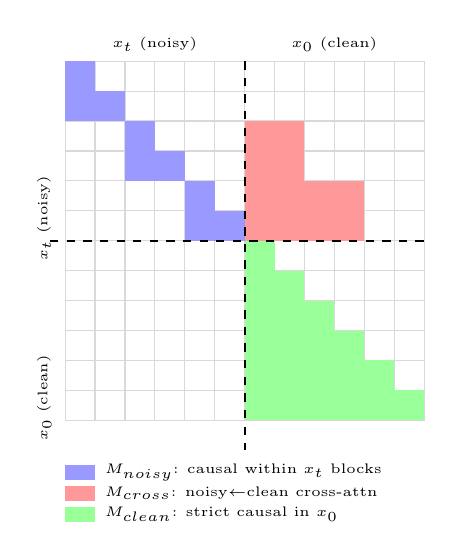
\begin{tikzpicture}[scale=0.38, every node/.style={font=\tiny}]
    % Grid size: 12x12 (block_size=2, n=6, total=12)
    % xt = positions 0-5, x0 = positions 6-11
    % Blocks: {0,1}, {2,3}, {4,5} for xt; {6,7}, {8,9}, {10,11} for x0

    % Draw grid
    \foreach \i in {0,...,11} {
        \foreach \j in {0,...,11} {
            \draw[gray!30] (\j, -\i) rectangle (\j+1, -\i+1);
        }
    }

    % M_BD: causal within xt blocks (use_regular_causal=True)
    % Block 0: (0,0)
    \fill[blue!40] (0,0) rectangle (1,1);
    % Block 0: (1,0), (1,1)
    \fill[blue!40] (0,-1) rectangle (1,0);
    \fill[blue!40] (1,-1) rectangle (2,0);
    % Block 1: (2,2)
    \fill[blue!40] (2,-2) rectangle (3,-1);
    % Block 1: (3,2), (3,3)
    \fill[blue!40] (2,-3) rectangle (3,-2);
    \fill[blue!40] (3,-3) rectangle (4,-2);
    % Block 2: (4,4)
    \fill[blue!40] (4,-4) rectangle (5,-3);
    % Block 2: (5,4), (5,5)
    \fill[blue!40] (4,-5) rectangle (5,-4);
    \fill[blue!40] (5,-5) rectangle (6,-4);

    % M_OBC: xt attends to x0 from previous blocks
    % xt block 1 (rows 2,3) attends to x0 block 0 (cols 6,7)
    \fill[red!40] (6,-2) rectangle (8,-1);
    \fill[red!40] (6,-3) rectangle (8,-2);
    % xt block 2 (rows 4,5) attends to x0 blocks 0,1 (cols 6,7,8,9)
    \fill[red!40] (6,-4) rectangle (10,-3);
    \fill[red!40] (6,-5) rectangle (10,-4);

    % M_BC: strict causal in x0 (use_regular_causal=True)
    \fill[green!40] (6,-6) rectangle (7,-5);
    \fill[green!40] (6,-7) rectangle (8,-6);
    \fill[green!40] (6,-8) rectangle (9,-7);
    \fill[green!40] (6,-9) rectangle (10,-8);
    \fill[green!40] (6,-10) rectangle (11,-9);
    \fill[green!40] (6,-11) rectangle (12,-10);

    % Separator lines
    \draw[thick, dashed] (6, 1) -- (6, -12);
    \draw[thick, dashed] (-0.5, -5) -- (12, -5);

    % Labels
    \node[above] at (3, 1) {$x_t$ (noisy)};
    \node[above] at (9, 1) {$x_0$ (clean)};
    \node[left, rotate=90] at (-0.7, -2.5) {$x_t$ (noisy)};
    \node[left, rotate=90] at (-0.7, -8.5) {$x_0$ (clean)};

    % Legend
    \fill[blue!40] (0, -13) rectangle (1, -12.5);
    \node[right] at (1, -12.75) {$M_\text{noisy}$: causal within $x_t$ blocks};
    \fill[red!40] (0, -13.7) rectangle (1, -13.2);
    \node[right] at (1, -13.45) {$M_\text{cross}$: noisy$\leftarrow$clean cross-attn};
    \fill[green!40] (0, -14.4) rectangle (1, -13.9);
    \node[right] at (1, -14.15) {$M_\text{clean}$: strict causal in $x_0$};
\end{tikzpicture}
\caption{\textbf{Strided DLLM (Ours).} Strict causal within $x_t$ blocks and strict causal in $x_0$.}
\label{fig:attn_mask_ours}
\end{subfigure}
\hfill
\begin{subfigure}[t]{0.48\textwidth}
\centering
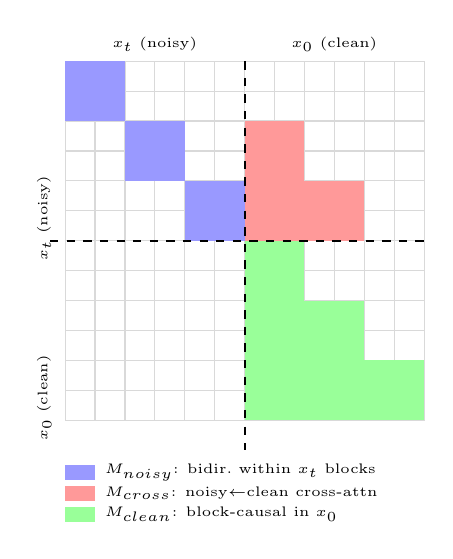
\begin{tikzpicture}[scale=0.38, every node/.style={font=\tiny}]
    % SDAR: bidirectional within blocks, block-causal in x0

    % Draw grid
    \foreach \i in {0,...,11} {
        \foreach \j in {0,...,11} {
            \draw[gray!30] (\j, -\i) rectangle (\j+1, -\i+1);
        }
    }

    % M_BD: bidirectional within xt blocks (SDAR)
    \fill[blue!40] (0,0) rectangle (2,1);
    \fill[blue!40] (0,-1) rectangle (2,0);
    \fill[blue!40] (2,-2) rectangle (4,-1);
    \fill[blue!40] (2,-3) rectangle (4,-2);
    \fill[blue!40] (4,-4) rectangle (6,-3);
    \fill[blue!40] (4,-5) rectangle (6,-4);

    % M_OBC: same as ours
    \fill[red!40] (6,-2) rectangle (8,-1);
    \fill[red!40] (6,-3) rectangle (8,-2);
    \fill[red!40] (6,-4) rectangle (10,-3);
    \fill[red!40] (6,-5) rectangle (10,-4);

    % M_BC: block-causal in x0 (SDAR)
    \fill[green!40] (6,-6) rectangle (8,-5);
    \fill[green!40] (6,-7) rectangle (8,-6);
    \fill[green!40] (6,-8) rectangle (10,-7);
    \fill[green!40] (6,-9) rectangle (10,-8);
    \fill[green!40] (6,-10) rectangle (12,-9);
    \fill[green!40] (6,-11) rectangle (12,-10);

    % Separator lines
    \draw[thick, dashed] (6, 1) -- (6, -12);
    \draw[thick, dashed] (-0.5, -5) -- (12, -5);

    % Labels
    \node[above] at (3, 1) {$x_t$ (noisy)};
    \node[above] at (9, 1) {$x_0$ (clean)};
    \node[left, rotate=90] at (-0.7, -2.5) {$x_t$ (noisy)};
    \node[left, rotate=90] at (-0.7, -8.5) {$x_0$ (clean)};

    % Legend
    \fill[blue!40] (0, -13) rectangle (1, -12.5);
    \node[right] at (1, -12.75) {$M_\text{noisy}$: bidir.\ within $x_t$ blocks};
    \fill[red!40] (0, -13.7) rectangle (1, -13.2);
    \node[right] at (1, -13.45) {$M_\text{cross}$: noisy$\leftarrow$clean cross-attn};
    \fill[green!40] (0, -14.4) rectangle (1, -13.9);
    \node[right] at (1, -14.15) {$M_\text{clean}$: block-causal in $x_0$};
\end{tikzpicture}
\caption{\textbf{SDAR (Block Diffusion).} Bidirectional within $x_t$ blocks and block-causal in $x_0$.}
\label{fig:attn_mask_sdar}
\end{subfigure}
\caption{\textbf{Attention mask comparison} for block size $N{=}2$, sequence length $L{=}6$. Input is $[x_t \,|\, x_0]$ (noisy $\|$ clean). Rows are query positions; columns are key positions. Our Strided DLLM (left) uses strict causal attention everywhere, preserving AR compatibility. SDAR (right) uses bidirectional attention within noisy blocks and block-causal attention in the clean region. The three mask components---$M_\text{noisy}$ (noisy self-attention), $M_\text{cross}$ (noisy$\leftarrow$clean cross-attention), $M_\text{clean}$ (clean self-attention)---are color-coded.}
\label{fig:attn_mask}
\end{figure*}

\section{Additional Experimental Details}
\label{app:details}

\section{Additional Results}
\label{app:results}
